\documentclass{article}

\usepackage{amsmath, amssymb}
\usepackage{tikz}
\usepackage{graphicx}
\usepackage{caption}
\usepackage[margin=1in, landscape]{geometry}
\usetikzlibrary{shapes, arrows, positioning, fit, calc}

\begin{document}

% ---------- Input Embedding -> (to MHA) ----------
\noindent
\resizebox{\linewidth}{!}{%
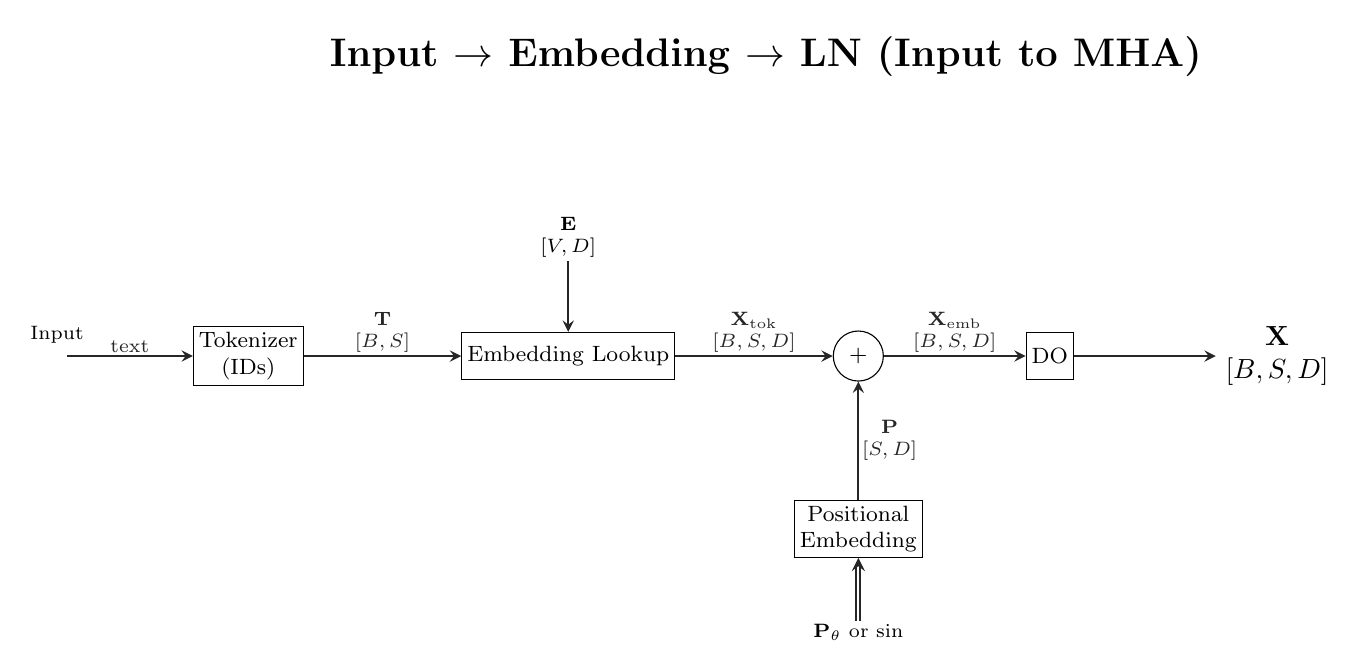
\begin{tikzpicture}[
  >=stealth,
  auxnode/.style={draw, rectangle, fill=white, minimum height=6mm, inner sep=2pt, font=\footnotesize, align=center},
  mulnode/.style={draw, circle, fill=white, minimum size=6mm, font=\footnotesize, align=center},
  addnode/.style={draw, circle, fill=white, minimum size=6mm, font=\footnotesize, align=center},
  flow/.style={->, thick, black!85},
  flow2/.style={->, double, thick, black!85},
  dimlabel/.style={font=\scriptsize, inner sep=1pt, align=center}
]

\node[font=\Large\bfseries] at (9, 3.8) {Input $\rightarrow$ Embedding $\rightarrow$ LN (Input to MHA)};

% nodes
\node (RawText) at (0,0) {};
\node[auxnode, align=center] (Tok)   [right=1.6cm of RawText] {Tokenizer\\(IDs)};
\node[auxnode, align=center] (Lookup)[right=2.0cm of Tok]     {Embedding Lookup};
\node[addnode, minimum size=6mm] (Sum) [right=2.0cm of Lookup] {+};
\node[auxnode, align=center] (PosE)  [below=1.5cm of Sum]  {Positional\\Embedding};
\node[auxnode] (Drop) [right=1.8cm of Sum] {DO};
\node (OUTPUT)   [align=center, right=1.8cm of Drop]   {$\mathbf{X}$\\$[B,S,D]$};

% parameter/const “double” edges
\node[dimlabel] (Eparam) [align=center, above=0.9cm of Lookup] {$\mathbf{E}$\\$[V,D]$};
\node[dimlabel] (Pparam) [align=center, below=0.8cm of PosE]   {$\mathbf{P}_{\theta}$ or sin};

% flows
\draw[flow] (RawText) -- (Tok) node[dimlabel, midway, above]
  {$\text{text}$};
\draw[flow] (Tok) -- (Lookup) node[dimlabel, midway, above]
  {$\mathbf{T}$\\$[B,S]$};

% Embedding matrix E
\draw[flow] (Eparam) -- (Lookup);

% Lookup -> Sum (token embeddings)
\draw[flow] (Lookup) -- (Sum) node[dimlabel, midway, above]
  {$\mathbf{X}_{\text{tok}}$\\$[B,S,D]$};

% Positional embedding path
\draw[flow] (PosE) -- (Sum) node[dimlabel, midway, right]
  {$\mathbf{P}$\\$[S,D]$};

% Optional: show P as parameter (sinusoidal/learned)
\draw[flow2] (Pparam) -- (PosE) ;

\draw[flow] (Sum) -- (Drop) node[dimlabel, midway, above]
  {$\mathbf{X}_{\text{emb}}$\\$[B,S,D]$};
\draw[flow] (Drop) -- (OUTPUT);

% labels for start and destination
\node[dimlabel, above=0.0cm of RawText] {Input};

\end{tikzpicture}%
}

\newpage
\renewcommand{\arraystretch}{1.2}
\small

% -------- Operations (Ops) --------
\begin{center}
\textbf{Operations (Ops)}
\begin{tabular}{llll}
\hline
\textbf{Abbrev} & \textbf{Name} & \textbf{Type / Shape} & \textbf{Notes} \\
\hline
Tokenizer & Tokenizer (IDs) & op & Maps raw text $\to$ integer ids $\mathbf{T}\in\mathbb{Z}^{[B,S]}$. \\
Embedding Lookup & Embedding Lookup & op & Gathers rows from $\mathbf{E}\in\mathbb{R}^{V\times D}$ using ids $\mathbf{T}$. \\
$+$ & Element-wise Add (dashed circle) & op & Adds token and positional embeddings; broadcasting over $B,S$ if needed. \\
DO & Dropout & op & Training-time stochastic dropout on $\mathbf{X}_{\text{emb}}$; identity at inference. \\
\textit{(none)} & Broadcast $\mathrm{BC}_{B,S}(\cdot)$ & op & Expands $[S,D]$ (or $[D]$) to $[B,S,D]$ across batch/sequence. \\
\hline
\end{tabular}
\end{center}

\vspace{0.8em}

% -------- Data Tensors (Values) --------
\begin{center}
\textbf{Data Tensors (Values)}
\begin{tabular}{llll}
\hline
\textbf{Symbol} & \textbf{Name} & \textbf{Shape} & \textbf{Notes} \\
\hline
text & Raw input text & — & Character/byte stream before tokenization. \\
$\mathbf{T}$ & Token ids & $[B,S]$ & Output of Tokenizer; integers in $\{0,\dots,V{-}1\}$. \\
$\mathbf{E}$ & Embedding matrix (params) & $[V,D]$ & Trainable; each vocab entry has a $D$-dim vector. \\
$\mathbf{X}_{\text{tok}}$ & Token embeddings & $[B,S,D]$ & $\mathrm{lookup}(\mathbf{E}, \mathbf{T})$. \\
$\mathbf{P}$ & Positional embedding & $[S,D]$ (or $[B,S,D]$) & Learned $\mathbf{P}_\theta$ \textbf{or} sinusoidal (fixed); broadcast to $[B,S,D]$. \\
$\mathbf{X}_{\text{emb}}$ & Sum of token+pos & $[B,S,D]$ & $\mathbf{X}_{\text{tok}} + \mathrm{BC}_{B,S}(\mathbf{P})$. \\
$\mathbf{X}$ & Input to MHA & $[B,S,D]$ & After dropout (DO); goes to LN/MHA stack. \\
$\mathbf{P}_\theta$ & Learned pos. params & matches $\mathbf{P}$ & Used when positions are trainable; otherwise “sin” denotes fixed sinusoidal. \\
\hline
\multicolumn{4}{l}{\textbf{Shape symbols:}\; $B$=batch size,\; $S$=sequence length,\; $D$=model dim,\; $V$=vocab size.} \\
\multicolumn{4}{l}{\textbf{Notes:}\; In practice, $\mathbf{P}$ may be pre-broadcast to $[B,S,D]$ or added per-token with implicit broadcasting.} \\
\hline
\end{tabular}
\end{center}

\end{document}
